\documentclass[12pt]{article}

\usepackage[margin=1in]{geometry}
\usepackage[T1]{fontenc}
\usepackage{lmodern}
\usepackage{microtype}
\usepackage{amsmath,amssymb,mathtools}
\usepackage{booktabs}
\usepackage{enumitem}
\usepackage{setspace}
\usepackage{xcolor}
\usepackage{tikz}
\usepackage{hyperref}
\usepackage{xurl}

\hypersetup{
  colorlinks=true,
  linkcolor=black,
  citecolor=black,
  urlcolor=blue,
  pdftitle={Proper Velocity: Distance on the Traveler's Clock},
  pdfauthor={Light-Meter Physics},
  pdfsubject={Proper velocity, celerity, relativistic momentum, and rapidity},
  pdfkeywords={special relativity, proper velocity, celerity, proper time, momentum, rapidity}
}

\onehalfspacing
\widowpenalty=10000
\clubpenalty=10000
\definecolor{ink}{HTML}{172E3D}
\definecolor{teal}{HTML}{126D77}
\definecolor{rust}{HTML}{B1533E}

\title{Proper Velocity:\\
Distance on the Traveler's Clock}
\author{Light-Meter Physics}
\date{Draft Manuscript}

\begin{document}

\maketitle

\begin{abstract}
Proper velocity, also called celerity, measures laboratory displacement per unit proper time along a massive particle's worldline. In one-dimensional motion in flat spacetime, the chain rule gives $u=\gamma v$, where $v$ is the velocity in a chosen inertial laboratory frame and $\gamma=dt/d\tau$. The same quantity simplifies relativistic momentum to $p=mu$ for fixed rest mass. Although $|u|$ can exceed $c$, the corresponding laboratory velocity remains subluminal: $v=u/\sqrt{1+(u/c)^2}$. An idealized constant-speed journey at $0.8c$ illustrates how the laboratory and traveler clocks assign different durations to the same displacement. These relations are standard special-relativistic kinematics. Proper velocity is not the speed measured in the traveler's instantaneous rest frame, and it does not by itself specify a force history or a realizable travel profile.
\end{abstract}

\noindent\textbf{Keywords:} special relativity, proper velocity, celerity, proper time, relativistic momentum, rapidity

\section{Introduction}
\label{sec:introduction}

For a moving particle, the same laboratory displacement can be compared with more than one measure of elapsed time. Dividing by laboratory coordinate time gives ordinary velocity. Dividing by the particle's own proper time gives proper velocity. The second ratio can be numerically larger than $c$, but it is not the speed of a signal or the velocity measured in the particle's instantaneous rest frame.

This manuscript defines proper velocity from the proper-time interval, derives its relation to ordinary velocity and relativistic momentum, and explains how to interpret its magnitude. The discussion uses flat spacetime, one inertial laboratory frame, and a massive particle with fixed rest mass. A simple constant-speed trip to Proxima Centauri illustrates the clock comparison; it is not a mission design or a model of acceleration and braking.

The quantity provides a useful bridge between kinematics and momentum. For fixed rest mass, $p=mu$, so the laboratory-time rate of change of proper velocity gives the relativistic three-force directly. This identity does not add a new interaction law. The rapidity relations at the end connect proper velocity to a standard parametrization of one-dimensional motion.

\section{One journey, two clocks}
\label{sec:kinematics}

Use inertial laboratory coordinates $(t,x)$ in one spatial dimension and metric signature $(+,-)$. Along a future-directed timelike worldline, the proper-time interval satisfies
\begin{equation}
  c^2\,d\tau^2=c^2\,dt^2-dx^2
  =c^2\,dt^2\left(1-\frac{v^2}{c^2}\right),
  \qquad v\equiv\frac{dx}{dt}.
  \label{eq:proper-time}
\end{equation}
For a massive particle, define the signed dimensionless laboratory velocity $\beta$ and Lorentz factor $\gamma$ by
\begin{equation}
  \beta\equiv\frac{v}{c},
  \qquad
  \gamma\equiv\frac{dt}{d\tau}
  =\frac{1}{\sqrt{1-\beta^2}}.
  \label{eq:beta-gamma}
\end{equation}
Thus $d\tau=dt/\gamma$: for the same pair of nearby events on the particle's path, the proper-time interval is smaller than the laboratory-time interval whenever $v\ne0$.

If the dimensionless inverse clock rate is denoted by $\delta\tau$, then for the inertial laboratory coordinates used here $\delta\tau\equiv dt/d\tau=\gamma$. This manuscript uses $\gamma$ below to distinguish the ratio from the elapsed proper-time interval $\Delta\tau$.

\begin{figure}[ht]
  \centering
  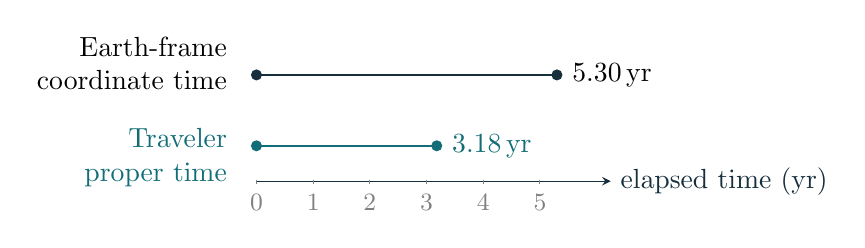
\begin{tikzpicture}[x=0.72cm,y=1cm,>=stealth]
    \draw[->,ink] (0,0)--(6.25,0) node[right] {elapsed time (yr)};
    \draw[thick,ink] (0,1.35)--(5.3,1.35);
    \fill[ink] (0,1.35) circle (2pt);
    \fill[ink] (5.3,1.35) circle (2pt);
    \node[anchor=east,align=right] at (-0.35,1.50) {Earth-frame\\coordinate time};
    \node[anchor=west] at (5.4,1.35) {$5.30\,\mathrm{yr}$};
    \draw[thick,teal] (0,0.45)--(3.18,0.45);
    \fill[teal] (0,0.45) circle (2pt);
    \fill[teal] (3.18,0.45) circle (2pt);
    \node[anchor=east,align=right,text=teal] at (-0.35,0.30) {Traveler\\proper time};
    \node[anchor=west,text=teal] at (3.28,0.45) {$3.18\,\mathrm{yr}$};
    \foreach \x/\lab in {0/0,1/1,2/2,3/3,4/4,5/5}{
      \draw[gray] (\x,0.02)--(\x,-0.03);
      \node[anchor=north,font=\small,text=gray] at (\x,-0.04) {\lab};
    }
  \end{tikzpicture}
  \caption{The same idealized $0.8c$ journey over $D\approx4.24\,\mathrm{ly}$ (see Sec.~\ref{sec:proxima}), with both elapsed-time bars drawn on a common scale. The upper bar is Earth-frame coordinate time; the lower bar is proper time along the traveler's worldline.}
  \label{fig:two-clocks}
\end{figure}

\section{Definition and chain-rule derivation}
\label{sec:definition}

Proper velocity is the rate of change of laboratory position with respect to the particle's proper time:
\begin{equation}
  u\equiv\frac{dx}{d\tau}.
  \label{eq:u-definition}
\end{equation}
Insert the laboratory time as an intermediate variable:
\begin{equation}
  u=\frac{dx}{dt}\frac{dt}{d\tau}=\gamma v.
  \label{eq:u-gamma-v}
\end{equation}
The derivation is the chain rule. The factor $\gamma$ converts the laboratory-time rate into a proper-time rate \cite{Tong}.

Proper velocity is frame-dependent because $dx$ and $dt$ refer to the chosen laboratory coordinates, while $d\tau$ is the invariant proper-time interval along the particle's path. It is not the velocity measured by an observer instantaneously comoving with the particle: that observer measures the particle to be at rest at that instant. The alternative name \emph{celerity} refers to the same quantity, not a different kind of velocity.

In three spatial dimensions the definition is $\mathbf u\equiv d\mathbf x/d\tau=\gamma\mathbf v$, where $\mathbf x$ and $\mathbf v$ are measured in the chosen laboratory frame. The scalar relations that follow are written for one-dimensional motion.

\section{Momentum in proper-velocity form}
\label{sec:momentum}

For fixed invariant rest mass $m$, one-dimensional relativistic momentum is
\begin{equation}
  p=\gamma mv.
  \label{eq:momentum}
\end{equation}
Combining this definition with Eq.~\eqref{eq:u-gamma-v} gives
\begin{equation}
  p=mu,
  \qquad
  \frac{u}{c}=\beta\,\delta\tau=\gamma\beta=\frac{p}{mc}.
  \label{eq:momentum-u}
\end{equation}
The relation $p=mu$ does not replace relativistic momentum with a new definition; it expresses the standard momentum in terms of proper velocity. In this form the mass-shell invariant becomes
\begin{equation}
  E^2-p^2c^2=m^2c^4,
  \qquad
  \gamma^2-\left(\frac{u}{c}\right)^2=1,
  \label{eq:mass-shell-u}
\end{equation}
where $E=\gamma mc^2$. The second equality displays the hyperbolic relation between the clock ratio and proper velocity.

\section{Force and the laboratory-time derivative}
\label{sec:force}

Relativistic three-force is defined as the laboratory-time derivative of momentum. For fixed rest mass, Eq.~\eqref{eq:momentum-u} therefore yields
\begin{equation}
  \mathbf F\equiv\frac{d\mathbf p}{dt}
  =m\frac{d\mathbf u}{dt}.
  \label{eq:force-u}
\end{equation}
This vector relation is exact in special relativity for constant $m$ \cite{Tong}. The derivative is with respect to laboratory coordinate time $t$, not proper time. Also, $d\mathbf u/dt$ is generally not the ordinary coordinate acceleration $d\mathbf v/dt$; Eq.~\eqref{eq:force-u} should not be read as the Newtonian formula $\mathbf F=m\mathbf a$ with $\mathbf a=d\mathbf v/dt$.

In one-dimensional motion, the distinction can be made explicit by differentiating $u=\gamma v$:
\begin{equation}
  \frac{du}{dt}
  =\frac{d(\gamma v)}{dv}\frac{dv}{dt}
  =\gamma^3 a_x,
  \qquad
  a_x\equiv\frac{dv}{dt},
  \qquad
  F_x=m\gamma^3a_x.
  \label{eq:longitudinal-force}
\end{equation}
As $v/c\to0$, $\gamma\to1$ and this reduces to $F_x\approx ma_x$. This kinematic identity does not extend the validity of a low-speed magnetic-dipole force model to relativistic motion. The scalar $\gamma^3$ relation is specific to one-dimensional motion and is not a general three-dimensional acceleration rule.

The identity is useful when a model already determines the force and one wants to track the momentum change. It does not determine the force, the mechanism supplying energy, or the time profile of an acceleration. Those require additional physical information about the system and its interaction with external fields.

\section{Worked example: a constant-speed leg at 0.8c}
\label{sec:proxima}

Consider an idealized one-dimensional journey over a laboratory-frame distance $D\approx4.24$ light-years, using the rounded Proxima Centauri distance reported by NASA \cite{NASAProxima}. Assume constant laboratory speed $v=0.8c=4c/5$ between fixed endpoints in one inertial Earth laboratory frame. Acceleration, braking, Earth orbital motion, relative stellar motion, and gravitational effects are omitted.

At this speed,
\begin{equation}
  \beta=\frac45,
  \qquad
  \gamma=\frac{1}{\sqrt{1-(4/5)^2}}=\frac53,
  \qquad
  u=\gamma v=\frac43c.
  \label{eq:proxima-speed-values}
\end{equation}
Because one light-year is the distance light travels in one year, the corresponding Earth-frame coordinate time is
\begin{equation}
  \Delta t=\frac{D}{v}
  =\frac{4.24\,\mathrm{ly}}{0.8c}
  =5.30\,\mathrm{yr}.
  \label{eq:proxima-lab-time}
\end{equation}
This laboratory duration uses synchronized clocks at the fixed endpoints.
At constant speed, $d\tau=dt/\gamma$ throughout the leg, so the traveler's elapsed proper time is
\begin{equation}
  \Delta\tau=\frac{\Delta t}{\gamma}
  =5.30\left(\frac35\right)\,\mathrm{yr}
  =3.18\,\mathrm{yr}.
  \label{eq:proxima-proper-time}
\end{equation}
For this constant-speed leg, laboratory displacement divided by traveler elapsed time equals the instantaneous proper velocity:
\begin{equation}
  \frac{D}{\Delta\tau}
  =\frac{4.24\,\mathrm{ly}}{3.18\,\mathrm{yr}}
  =\frac43c.
  \label{eq:proxima-average}
\end{equation}
The ratio does not describe a signal traveling at $4c/3$. It uses laboratory distance in the numerator and the traveler's proper time in the denominator. The Earth-frame elapsed time is coordinate time between departure and arrival events, not the time at which a distant observer receives light announcing the arrival. The distance is a rounded astronomical input rather than a precise future trajectory or mission distance.

The same trip can be checked using the traveler's inertial frame. At departure, the simultaneous separation of the laboratory endpoints in that frame is length-contracted:
\begin{equation}
  D'=\frac{D}{\gamma}=2.544\,\mathrm{ly}\approx2.54\,\mathrm{ly},
  \qquad
  \frac{D'}{0.8c}=3.18\,\mathrm{yr}.
  \label{eq:contracted-distance}
\end{equation}
The destination approaches at $0.8c$ across this contracted separation, reaching the traveler after $3.18$ years. Here $D'$ is the simultaneous separation of the endpoints in the traveler's frame. The traveler's departure and arrival events occur at the same ship coordinate, so the ship's displacement between those events in that frame is zero; it is not $D'$.

\section{Comparing ordinary and proper velocity}
\label{sec:comparison}

Equation~\eqref{eq:momentum-u} gives $u/c=\gamma\beta$. The table collects representative speeds, including the point where the proper-velocity magnitude first equals $c$. Solving $|\gamma\beta|=1$ gives
\begin{equation}
  \frac{\beta^2}{1-\beta^2}=1
  \quad\Longrightarrow\quad
  |\beta|=\frac{1}{\sqrt2},
  \qquad |v|=\frac{c}{\sqrt2}\approx0.7071c.
  \label{eq:threshold}
\end{equation}
\begin{table}[ht]
  \centering
  \small
  \begin{tabular}{@{}ccc@{}}
    \toprule
    $\beta=v/c$ & $\gamma$ & $u/c=\gamma\beta$ \\
    \midrule
    $0$ & $1$ & $0$ \\
    $0.6000$ & $1.2500$ & $0.7500$ \\
    $1/\sqrt2\approx0.7071$ & $\sqrt2$ & $1$ \\
    $0.8000$ & $5/3\approx1.6667$ & $4/3\approx1.3333$ \\
    $0.9000$ & $2.2942$ & $2.0647$ \\
    $0.9900$ & $7.0888$ & $7.0179$ \\
    \bottomrule
  \end{tabular}
  \caption{Ordinary velocity, Lorentz factor, and proper velocity. Decimal entries are rounded to four places from the exact formulas, rather than calculated from other rounded table entries.}
  \label{tab:velocity-comparison}
\end{table}

The table shows that $u$ can pass $c$ while $v$ remains below $c$. This follows directly by solving Eq.~\eqref{eq:u-gamma-v} for the laboratory velocity:
\begin{equation}
  v=\frac{u}{\sqrt{1+(u/c)^2}}.
  \label{eq:v-from-u}
\end{equation}
For every finite signed $u$, $|v|<c$. Only in the limit $|u|\to\infty$ does $|v|$ approach $c$.

\begin{figure}[ht]
  \centering
  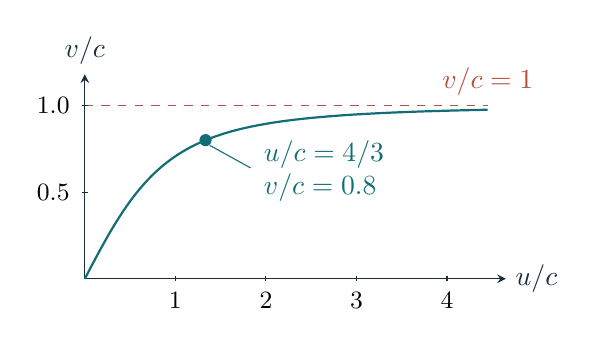
\begin{tikzpicture}[x=1.15cm,y=2.2cm,>=stealth]
    \draw[->,ink] (0,0)--(4.65,0) node[right] {$u/c$};
    \draw[->,ink] (0,0)--(0,1.18) node[above] {$v/c$};
    \draw[dashed,rust] (0,1)--(4.45,1) node[right,above] {$v/c=1$};
    \draw[thick,teal,domain=0:4.45,samples=120,smooth]
      plot ({\x},{\x/sqrt(1+\x*\x)});
    \foreach \x in {1,2,3,4}{
      \draw[ink] (\x,0.015)--(\x,-0.015);
      \node[anchor=north,font=\small] at (\x,-0.025) {$\x$};
    }
    \foreach \y in {0.5,1.0}{
      \draw[ink] (0.035,\y)--(-0.035,\y);
      \node[anchor=east,font=\small] at (-0.06,\y) {$\y$};
    }
    \fill[teal] (1.3333,0.8) circle (2.2pt);
    \draw[teal] (1.38,0.77)--(1.83,0.64);
    \node[anchor=west,teal,align=left] at (1.87,0.62)
      {$u/c=4/3$\\$v/c=0.8$};
  \end{tikzpicture}
  \caption{Ordinary velocity as a function of proper velocity. The curve approaches, but never reaches, the light-speed line for finite $u$.}
  \label{fig:velocity-map}
\end{figure}

\section{Rapidity and the mass-shell hyperbola}
\label{sec:rapidity}

For one-dimensional motion, define rapidity $\eta=\operatorname{artanh}\beta$. Then
\begin{equation}
  \beta=\tanh\eta,
  \qquad
  \gamma=\cosh\eta,
  \qquad
  \frac{u}{c}=\gamma\beta=\sinh\eta.
  \label{eq:rapidity-relations}
\end{equation}
The identity $\cosh^2\eta-\sinh^2\eta=1$ reproduces the mass-shell relation in Eq.~\eqref{eq:mass-shell-u}. Rapidity therefore parametrizes the future massive-particle branch in the plane with horizontal coordinate $\gamma$ and vertical coordinate $u/c$, connecting proper velocity to the standard hyperbolic description of one-dimensional motion \cite{Tong}.

\begin{figure}[ht]
  \centering
  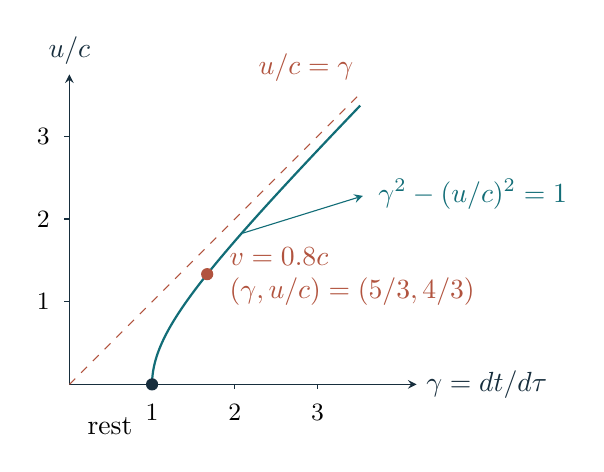
\begin{tikzpicture}[x=1.05cm,y=1.05cm,>=stealth]
    \draw[->,ink] (0,0)--(4.2,0) node[right] {$\gamma=dt/d\tau$};
    \draw[->,ink] (0,0)--(0,3.75) node[above] {$u/c$};
    \draw[dashed,rust] (0,0)--(3.55,3.55)
      node[above left] {$u/c=\gamma$};
    \draw[thick,teal,domain=0:0.96,samples=120,smooth]
      plot ({1/sqrt(1-\x*\x)},{\x/sqrt(1-\x*\x)});
    \fill[ink] (1,0) circle (2.2pt);
    \node[anchor=north east] at (0.88,-0.28) {rest};
    \fill[rust] (1.6667,1.3333) circle (2.2pt);
    \node[anchor=west,rust,align=left] at (1.82,1.3)
      {$v=0.8c$\\$(\gamma,u/c)=(5/3,4/3)$};
    \foreach \x in {1,2,3}{
      \draw[ink] (\x,0)--(\x,-0.06);
      \node[anchor=north,font=\small] at (\x,-0.12) {$\x$};
    }
    \foreach \y in {1,2,3}{
      \draw[ink] (0,\y)--(-0.06,\y);
      \node[anchor=east,font=\small] at (-0.12,\y) {$\y$};
    }
    \draw[teal,->] (2.1,1.83)--(3.55,2.28);
    \node[anchor=west,teal] at (3.62,2.3)
      {$\gamma^2-(u/c)^2=1$};
  \end{tikzpicture}
  \caption{The curve is the nonnegative-momentum portion of the future branch of the massive-particle mass shell. The null line is an asymptote, not a finite massive-particle state. Axes use equal units.}
  \label{fig:mass-shell}
\end{figure}

The dashed line $u/c=\gamma$ corresponds formally to $\beta=1$ and is approached only as $\eta\to\infty$. A photon has $d\tau=0$ along its null worldline, so $dx/d\tau$ is undefined as a proper velocity. The null line is an asymptote of the massive-particle hyperbola, not a finite massive-particle state.

\section{Interpretive limits}
\label{sec:limits}

The derivations establish a useful set of standard identities, subject to their assumptions:
\begin{itemize}[leftmargin=*]
  \item Proper velocity refers to laboratory displacement per particle proper time. It depends on the chosen laboratory frame and is not the particle's velocity measured in its own instantaneous rest frame.
  \item A finite proper velocity, including one with magnitude greater than $c$, corresponds to a subluminal laboratory velocity for a massive particle.
  \item The force identity $\mathbf F=m\,d\mathbf u/dt$ assumes fixed rest mass and uses laboratory coordinate time. It does not specify a force mechanism or an acceleration history.
  \item The Proxima Centauri calculation is an ideal constant-speed leg between fixed endpoints. It omits acceleration, braking, orbital motion, relative stellar motion, and gravity.
  \item Neither the ratio $D/\Delta\tau$ in the constant-speed example nor proper velocity generally represents a signal speed.
  \item Photons have no proper-time parameter and are not finite states on the massive-particle proper-velocity hyperbola.
\end{itemize}

\section{Conclusion}
\label{sec:conclusion}

Proper velocity is defined by $u=dx/d\tau$, using laboratory position and traveler proper time. The chain rule gives $u=\gamma v$, and relativistic momentum for fixed rest mass becomes $p=mu$. These relations explain both the utility of celerity and why its magnitude can exceed $c$: it combines a frame-dependent displacement with a different time parameter, while the associated laboratory speed remains $|v|<c$ for every finite $u$.

The idealized $0.8c$ example illustrates the clock distinction, not a practical travel profile. Rapidity places the same relations on the mass-shell hyperbola, and the force identity follows directly from momentum when rest mass is fixed. Together these are standard kinematic tools, not a new dynamical law.

\appendix
\clearpage

\section{Finite intervals and variable speed}
\label{app:finite-intervals}

The differential definition $u=dx/d\tau$ does not imply that a finite displacement divided by a finite proper-time interval always equals the instantaneous proper velocity. Integrating along a one-dimensional worldline gives
\begin{equation}
  \Delta x=\int_{\tau_1}^{\tau_2}u(\tau)\,d\tau,
  \qquad
  \frac{\Delta x}{\Delta\tau}
  =\frac{1}{\Delta\tau}\int_{\tau_1}^{\tau_2}u(\tau)\,d\tau,
  \qquad \Delta\tau=\tau_2-\tau_1.
  \label{eq:proper-time-average}
\end{equation}
Thus $\Delta x/\Delta\tau$ is the proper-time average of the signed proper velocity. If the particle reverses direction, this is net displacement per proper time; path length per proper time instead uses $|u|$ inside the integral. For the constant-speed, fixed-direction leg in Sec.~\ref{sec:proxima}, $u$ is constant and the finite ratio $D/\Delta\tau$ equals $u$.

\section{The proper-velocity identity from the mass shell}
\label{app:algebra}

Starting from $\gamma^2(1-\beta^2)=1$ and $u/c=\gamma\beta$,
\begin{equation}
  \gamma^2-\left(\frac{u}{c}\right)^2
  =\gamma^2(1-\beta^2)=1.
  \label{eq:app-hyperbola}
\end{equation}
Since $\gamma>0$, this implies $\gamma=\sqrt{1+(u/c)^2}$. Substituting into $u=\gamma v$ gives
\begin{equation}
  v=\frac{u}{\gamma}
   =\frac{u}{\sqrt{1+(u/c)^2}}.
  \label{eq:app-inverse}
\end{equation}
Setting $|u|=c$ in $|u|/c=\gamma|\beta|$ gives $\beta^2/(1-\beta^2)=1$, hence $|\beta|=1/\sqrt2$.

\clearpage

\begin{thebibliography}{9}
\small
\setstretch{1.0}
\raggedright
\urlstyle{same}

\bibitem{Tong}
D. Tong,
\emph{Dynamics and Relativity},
Chapter 7, §§7.3.2 and 7.4.1--7.4.5,
lecture notes, University of Cambridge,
available at \href{https://davidtong.org/teaching/dynamics-and-relativity/}{davidtong.org/teaching/dynamics-and-relativity/}.

\bibitem{NASAProxima}
NASA Science,
``Sun: Facts,'' section ``Size and Distance,''
Proxima Centauri distance stated as approximately $4.24$ light-years,
accessed 4 November 2026,
available at \href{https://science.nasa.gov/sun/facts/}{science.nasa.gov/sun/facts/}.

\end{thebibliography}

\end{document}